%Este trabalho está licenciado sob a Licença Atribuição-CompartilhaIgual 4.0 Internacional Creative Commons. Para visualizar uma cópia desta licença, visite http://creativecommons.org/licenses/by-sa/4.0/deed.pt_BR ou mande uma carta para Creative Commons, PO Box 1866, Mountain View, CA 94042, USA.

\chapter{Equações Diferenciais Parciais}\label{cap_edp}
\thispagestyle{fancy}

Neste capítulo, estudamos alguns tópicos fundamentais da aplicação do Método de Diferenças Finitas (MDF) para a solução numérica de Equações Diferenciais Parciais (EDPs).

\section{Equação de Poisson}\label{cap_edp_sec_poisson}

Consideramos a \hlemph{equação de Poisson}{\poisson} (ou \emph{equação de Laplace}{\laplace} heterogênea) no domínio retangular $D = (a, b)\times (c, d)$ com condições de contorno de Dirichlet homogêneas
\begin{subequations}\label{cap_edp_sec_poisson:eq:prob}\hleq
  \begin{align}
    &\Delta u = f(x, y), ~(x, y)\in D, \label{cap_edp_sec_poisson:eq:prob_eq}\\
    &u(x,y) = 0, ~\p D,\label{cap_edp_sec_poisson:eq:prob_bc}
  \end{align}
\end{subequations}
onde $u = u(x,y)$ é a incógnita, $\Delta u := u_{xx} + u_{yy}$ e $\p D$ é a fronteira do domínio $D$.

\hl{A aplicação do Método de Diferenças Finitas para resolver este problema consiste dos} mesmos \hl{passos} usados para resolver problemas de valores de contorno (consulte Seção~\ref{cap_pvc_sec_mdf}), a saber\hl{: 1. discretização do domínio, 2. discretização das equações, 3. resolução do problema discreto}.

\begin{flushleft}
  \hlemph{1. Discretização do Domínio (Malha).}
\end{flushleft}

Tratando-se do domínio retangular $\overline{D} = [a, b]\times [c, d]$, podemos construir uma malha do produto cartesiano de partições uniformes dos intervalos $[a, b]$ e $[c, d]$. Ou seja, tomamos
\begin{subequations}
  \begin{align}
    x_{i} &:= a + (i-1)h_x,\\
    y_{j} &:= c + (j-1)h_y,  
\end{align}
\end{subequations}
com $i = 1, 2, \dotsc, n_x+1$, $j = 1, 2, \dotsc, n_y+1$, sendo $n_x$ e $n_y$ o número de subintervalos escolhidos para as partições, respectivamente, e os passos $h_x = (b-a)/n_x$ e $h_y=(d-c)/n_y$. O tamanho da malha é definido por $h := \max\{h_x, h_y\}$.

\begin{figure}[H]
  \centering
  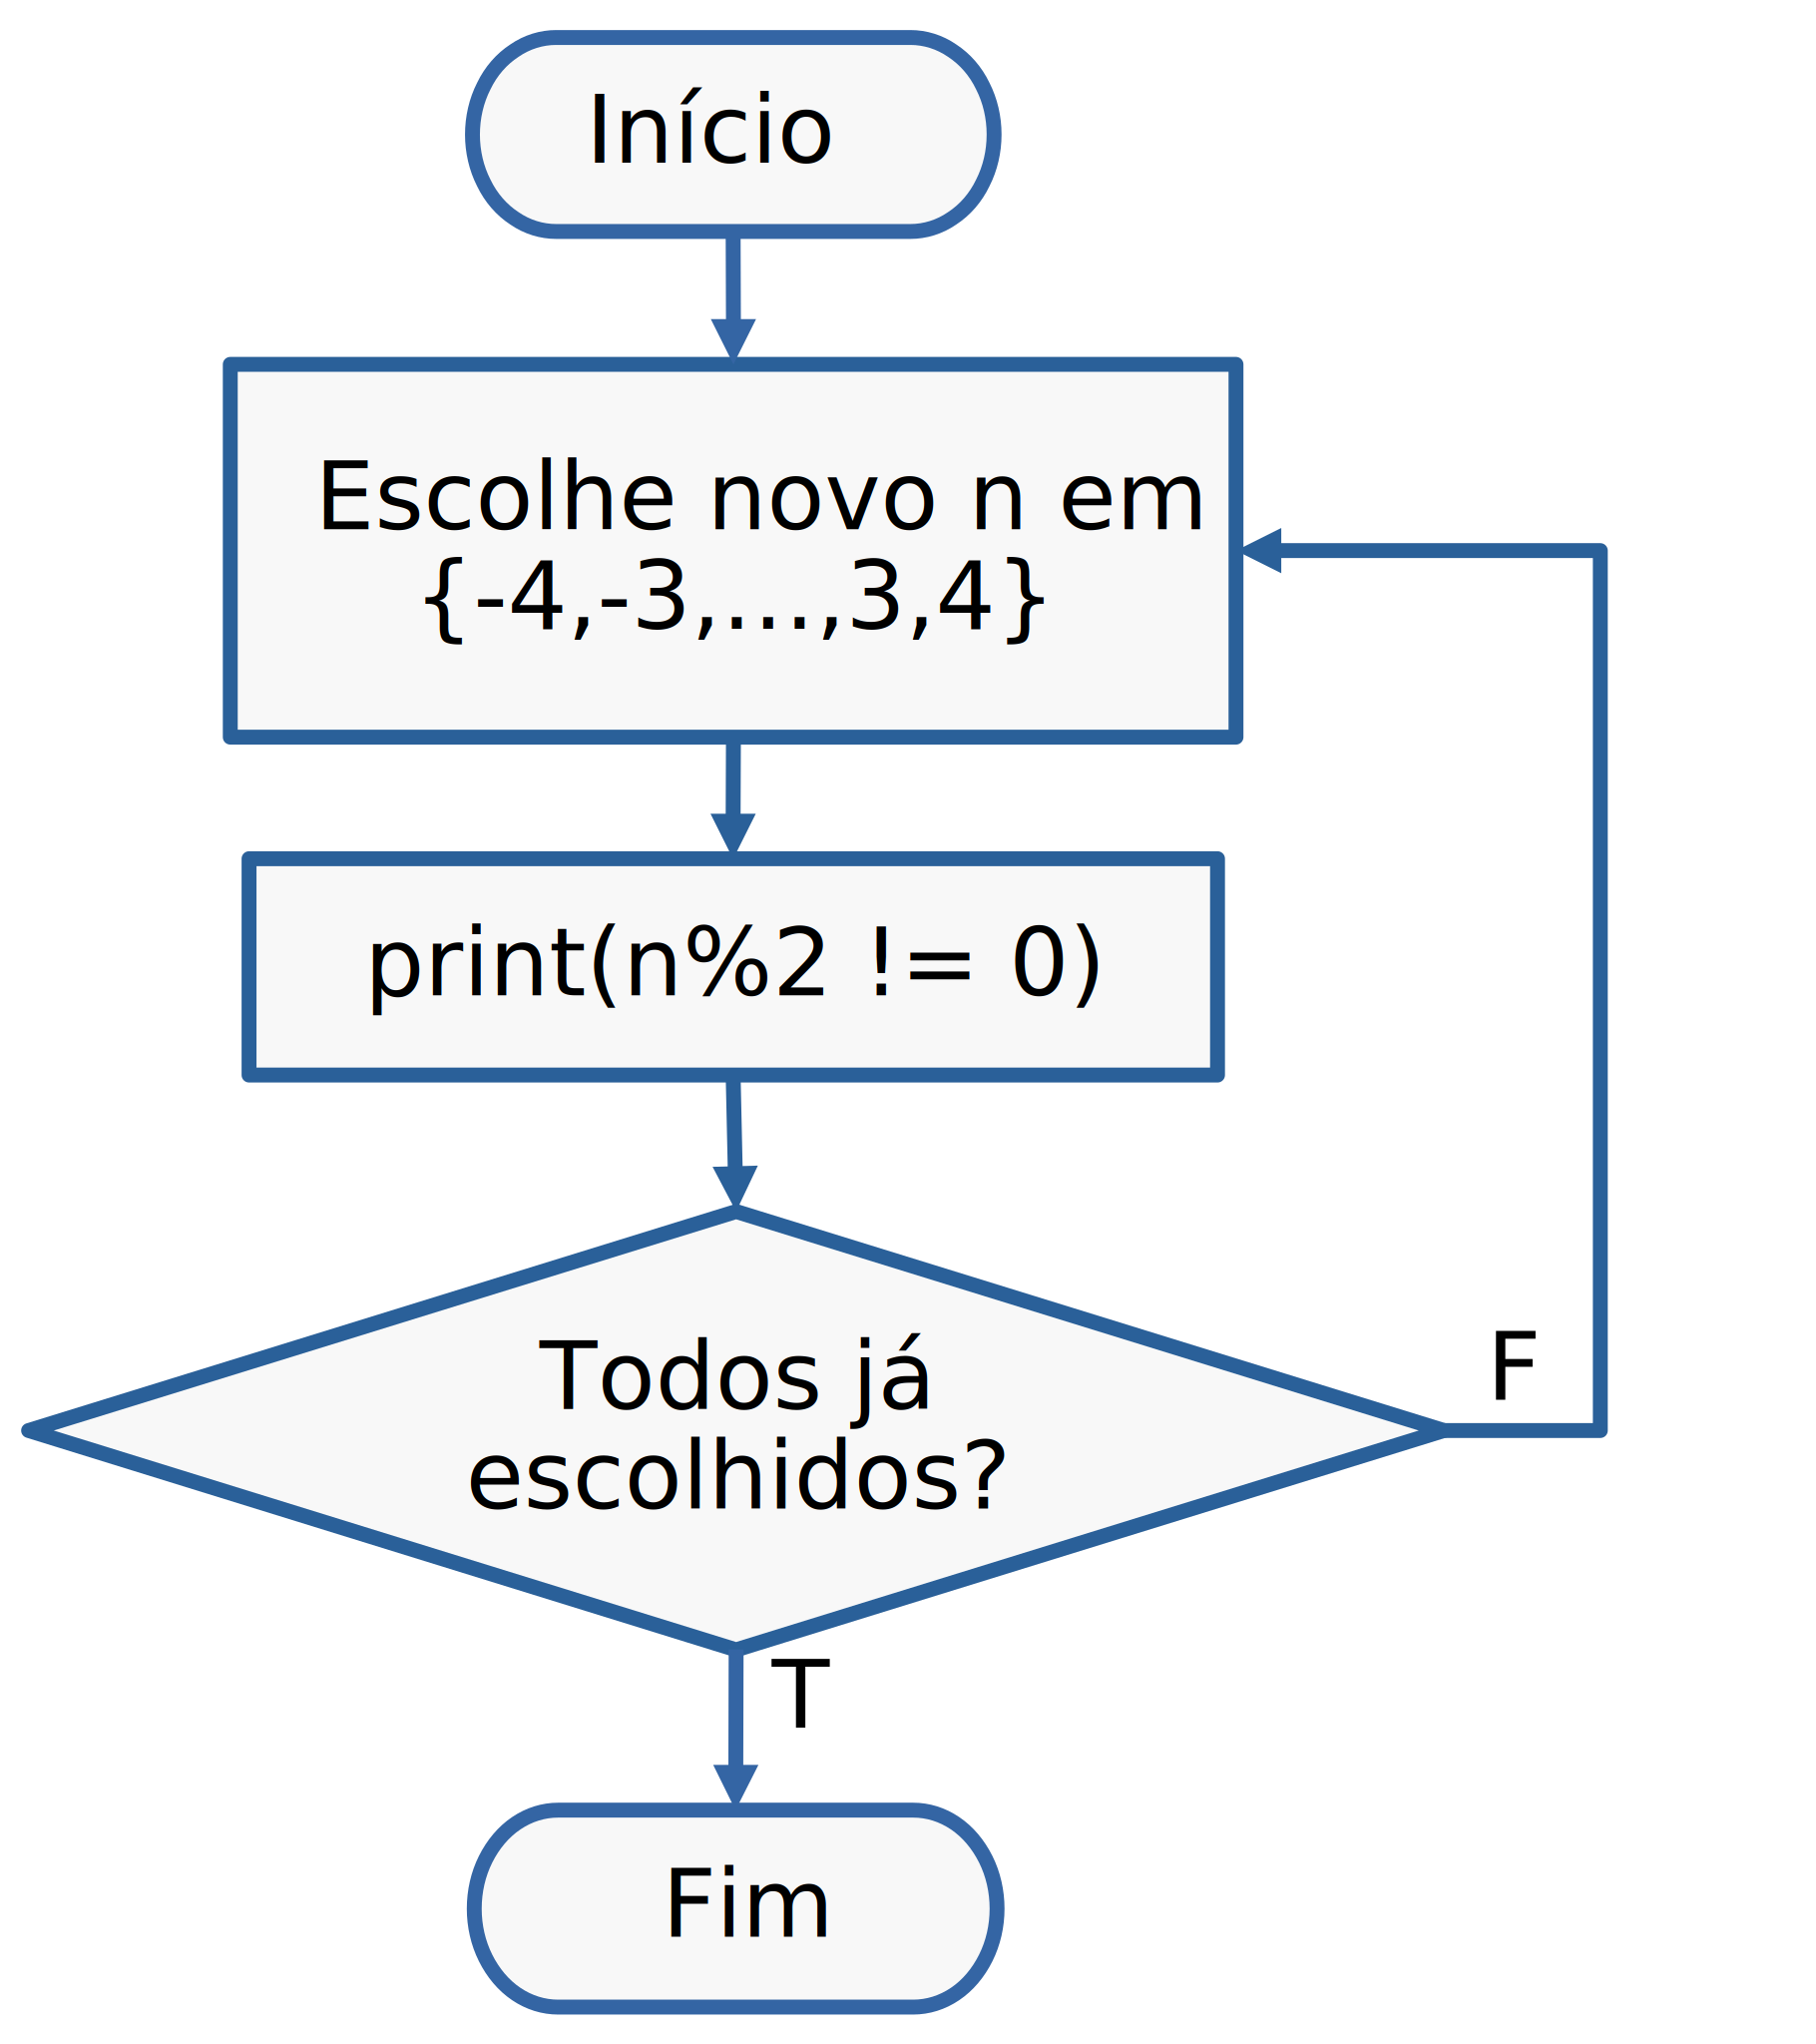
\includegraphics[width=0.8\textwidth]{./cap_edp/dados/figMalha2D/fig}
  \caption{Malha bidimensional.}
  \label{cap_edp_sec_poisson:fig:malha2D}
\end{figure}

O produto cartesiano das partições em $x$ e $y$ nos fornece uma partição do domínio $\overline{D}$ da forma
\begin{equation}
  P(\overline{D}) = \{(x_1, y_1), (x_1, y_2), \dotsc, (x_i, y_j), \dotsc, (x_{n_x}, y_{n_y})\},
\end{equation}
cujos nodos $(x_i, y_j)$ podem ser enumerados (indexados) por $k = i + (j-1)(n_x+1)$.  Por simplicidade, no decorrer do texto, assumiremos $n_x=n_y=:n$ e, por conseguinte, $h_x=h_y=h$ e temos a \hlemph{enumeração}
\begin{equation}\label{cap_edp_sec_poisson:eq:enum}\hleq
  k = i + (j-1)(n+1).
\end{equation}
Consulte a Figura~\ref{cap_edp_sec_poisson:fig:malha2D}.

\begin{flushleft}
  \hlemph{2. Discretização das Equações.}
\end{flushleft}

Usando a \href{https://notaspedrok.com.br/notas/MatematicaNumericaII/cap_deriv_sec_d2f.html}{fórmula de diferenças finitas central} de ordem $h^2$ para a segunda derivada, temos
\begin{align}
  u_{xx}(x,y) &= \frac{u(x+h,y)-2u(x,y)+u(x-h,y)}{h^2} + O(h^2),\\
  u_{yy}(x,y) &= \frac{u(x,y+h)-2u(x,y)+u(x,y-h)}{h^2} + O(h^2).
\end{align}
Daí, denotando $u_{ij}\approx u(x_i, y_j)$ temos
\begin{align}
  u_{xx}(x_i,y_j) &= \frac{u_{i+1,j}-2u_{i,j}+u_{i-1,j}}{h^2} + O(h^2),\\
  u_{yy}(x_i,y_j) &= \frac{u_{i,j+1}-2u_{i,j}+u_{i,j-1}}{h^2} + O(h^2).  
\end{align}
Então, da Eq.~\ref{cap_edp_sec_poisson:eq:prob_eq} temos
\begin{equation}
  \begin{aligned}
    &\frac{u_{i+1,j}-2u_{i,j}+u_{i-1,j}}{h^2}\\
    &\qquad + \frac{u_{i,j+1}-2u_{i,j}+u_{i,j-1}}{h^2} + O(h^2) = f(x_i,y_j).
\end{aligned}
\end{equation}
Agora, com base na enumeração \eqref{cap_edp_sec_poisson:eq:enum} denotamos $u_k := u_{i+(j-1)(n+1)}$, desprezando o erro de truncamento e rearranjando os termos, obtemos
\begin{equation}\label{cap_edp_sec_poisson:eq:mdf_ni}\hleq
  \frac{1}{h^2}u_{k-n} + \frac{1}{h^2}u_{k-1} -\frac{4}{h^2}u_{k} + \frac{1}{h^2}u_{k+1} + \frac{1}{h^2}u_{k+n} = f_k,
\end{equation}
para $k = i + (j+1)(n+1)$ com $i,j=2, 3, \dotsc, n$ (nodos internos). Isto é, esta última expressão nos fornece um sistema de $(n-1)^2$ equações para $(n+1)^2$ incógnitas $\pmb{u} = (u_k)_{k=1}^{(n+1)^2}$. Para fechar o sistema, usamos as condições de contorno \eqref{cap_edp_sec_poisson:eq:prob_bc}
\begin{equation}\label{cap_edp_sec_poisson:eq:mdf_nb}\hleq
  u_k = 0
\end{equation}
para $k = i + (j+1)(n+1)$ com $i=1, n+1$ e $j=1, 2, \dotsc, n+1$, ou $i=2,3,\dotsc, n$ e $j=1, n+1$.

Com isso, o \hlemph{problema discreto} obtido da aplicação do MDF \hl{consiste no sistema linear de $(n+1)^2\times (n+1)^2$ {\eqref{cap_edp_sec_poisson:eq:mdf_ni}}-{\eqref{cap_edp_sec_poisson:eq:mdf_nb}}}.


\begin{flushleft}
  \hlemph{3. Resolução do Problema Discreto.}
\end{flushleft}

O problema discreto \eqref{cap_edp_sec_poisson:eq:mdf_ni}-\eqref{cap_edp_sec_poisson:eq:mdf_nb} pode ser escrito na forma matricial
\begin{equation}\label{cap_edp_sec_poisson:eq:sis}\hleq
  A\pmb{u} = \pmb{b},
\end{equation}
onde o vetor da incógnitas é $\pmb{u}=(u_k)_{k=1}^{(n+1)^2}$. A matriz dos coeficientes $A = [a_{l,m}]_{l,m=1}^{(n+1)^2,(n+1)^2}$ e o vetor dos termos contantes $\pmb{b} = (b_{k})_{k=1}^{(n+1)^2}$ têm elementos não nulos
\begin{equation}
  \begin{aligned}
    &i=1, n+1, ~j=1, 2, \dotsc, n+1:\\
    &\qquad a_{k,k} = 1,\\
    &\qquad b_k = 0,\\
  \end{aligned}
\end{equation}
\begin{equation}
  \begin{aligned}
    &i=1, 2, \dotsc, n+1, ~j=1, n+1:\\
    &\qquad a_{k,k} = 1,\\
    &\qquad b_k = 0,\\
  \end{aligned}
\end{equation}
\begin{equation}
  \begin{aligned}
    &i,j=2, 3, \dotsc, n &:\\
    &\qquad a_{k,k-n} = \frac{1}{h^2},\\
    &\qquad a_{k,k-1} = \frac{1}{h^2},\\
    &\qquad a+{k,k} = -\frac{4}{h^2},\\
    &\qquad a_{k,k+1} = \frac{1}{h^2},\\
    &\qquad a_{k,k+n} = \frac{1}{h^2},\\
    &\qquad b_{k} = f(x_i, y_j).
  \end{aligned}
\end{equation}
Assim sendo, basta empregarmos um método apropriado para resolver o sistema linear \eqref{cap_edp_sec_poisson:eq:sis} para obter a solução aproximada de $u$ nos nodos $(x_i, y_j)$.

\begin{ex}\label{cap_edp_sec_poisson:ex:poisson}
  Consideramos o seguinte problema
  \begin{subequations}
    \begin{align}
      &\Delta u = -2\pi^2\sen(\pi x)\sen(\pi y),~(x, y)\in (0, 1)^2,\\
      &u = 0, ~(x,y)\in\p D.
    \end{align}
\end{subequations}
A solução exata é $u(x,u) = \sen(\pi x)\sen(\pi y)$.

A Figura~\ref{cap_edp_sec_poisson:fig:ex_poisson_a} mostra o gráfico de superfície da solução aproximada obtida pelo MDF com $h = 10^{-1}$. A Figura~\ref{cap_edp_sec_poisson:fig:ex_poisson_b} mostra a comparação entre os gráficos de contorno das soluções numérica e exata (linhas brancas).

\begin{figure}[H]
  \centering
  \includegraphics[width=0.8\textwidth]{./cap_edp/dados/fig_ex_poisson/fig_surface}
  \caption{Solução aproximada do problema de Poisson do Exemplo~\ref{cap_edp_sec_poisson:ex:poisson}.}
  \label{cap_edp_sec_poisson:fig:ex_poisson_a}
\end{figure}

\begin{figure}[H]
  \centering
  \includegraphics[width=0.8\textwidth]{./cap_edp/dados/fig_ex_poisson/fig_contour}
  \caption{Comparação das soluções numérica e exata (isolinhas brancas) do Exemplo~\ref{cap_edp_sec_poisson:ex:poisson}.}
  \label{cap_edp_sec_poisson:fig:ex_poisson_b}
\end{figure}

\begin{lstlisting}[caption=mdf\_poisson.py]
import numpy as np
import numpy.linalg as npla

# malha
n = 10
h = 1./n
xx = np.linspace(0., 1., n+1)
yy = np.linspace(0., 1., n+1)

# rhs
def f(x,y):
    return -2*np.pi**2*np.sin(np.pi*x)*np.sin(np.pi*y)

# problema discreto
A = np.zeros(((n+1)**2, (n+1)**2))
b = np.empty((n+1)**2)

# c.c.
for j in range(n+1):
    # i = 0
    k = j*(n+1)
    A[k,k] = 1.
    b[k] = 0.
    # i = n
    k = n + j*(n+1)
    A[k,k] = 1.
    b[k] = 0.

for i in range(1,n):
    # j = 0
    k = i
    A[k,k] = 1.
    b[k] = 0.
    # j = n
    k = i + n*(n+1)
    A[k,k] = 1.
    b[k] = 0.

# pts internos
for i in range(1,n):
    for j in range(1,n):
        k = i + j*(n+1)
        A[k,k-n-1] = 1./h**2
        A[k,k-1] = 1./h**2
        A[k,k] = -4./h**2
        A[k,k+1] = 1./h**2
        A[k,k+n+1] = 1./h**2
        b[k] = f(xx[i],yy[j])

# resol p.d.
u = npla.solve(A, b)
\end{lstlisting}

\end{ex}

\subsection{Exercícios}

\begin{exer}
  Use o MDF para encontrar uma solução aproximada do seguinte problema de Poisson
  \begin{subequations}
    \begin{align}
      &\Delta u = -2\pi^2\sen(\pi x)\sen(\pi y),~(x, y)\in D=(-1, 1)^2,\\
      &u = 0, ~(x,y)\in\p D.
    \end{align}
\end{subequations}
A solução exata é $u(x,y) = \sen(\pi x)\sen(\pi y)$. Faça uma comparação gráfica entre as soluções numérica e exata no caso de $h = 10^{-1}$ (malha uniforme). Compare o erro $\varepsilon_h := \|\tilde{\pmb{u}}_h -\pmb{u}\|_2$ para $n = 10, 20, 40, 80, 160$ (número de subintervalos na malha uniforme). A taxa de convergência é a esperada? Justifique sua resposta.
\end{exer}

\begin{exer}
  Use o MDF para encontrar uma solução aproximada do seguinte problema de Laplace
  \begin{subequations}
    \begin{align}
      &\Delta u = 0,~(x, y)\in (0, 1)^2,\\
      &u(0,y) = u(1,y) = y^2-y, ~0\leq y\leq 1,\\
      &u(x,0) = u(x,1) = x-x^2, ~0\leq x\leq 1.
    \end{align}
\end{subequations}
A solução exata é $u(x,y) = x-x^2 + y^2-y$. Faça uma comparação gráfica entre as soluções numérica e exata no caso de $h = 10^{-1}$. Compare o erro $\varepsilon_h := \|\tilde{\pmb{u}}_h -\pmb{u}\|_2$ para $n = 10, 20, 40, 80, 160$ (número de subintervalos na malha uniforme).
\end{exer}

\begin{exer}
  Considere o problema
  \begin{subequations}
    \begin{align}
      &\Delta u = -2\pi^2\sen(\pi x)\sen(\pi y),~(x, y)\in (0, 1)^2,\\
      &u(0,y) = 0, ~0\leq y\leq 1,\\
      &u_x(1,y) = 0, ~0\leq y\leq 1,\\
      &u(x,0) = u(x,1) = 0, ~0\leq x\leq 1.
    \end{align}
\end{subequations}
A solução exata é $u(x,y) = \sen(\pi x)\sen(\pi y)$. Com uma malha uniforme, obtenha uma solução aproximada com o MDF empregando, na fronteira com condições de Neumann{\neumann}:
\begin{enumerate}[a)]
\item $D_{-,h}$ fórmulas diferença regressiva de ordem $h$.
\item $D_{-,h^2}$ diferença regressiva de ordem $h^2$.
\end{enumerate}
Compare a taxa de convergência do erro $\varepsilon_h := \|\tilde{\pmb{u}}_h -\pmb{u}\|_2$ entre essas duas formulações.
\end{exer}

\begin{exer}
  Considere o problema
  \begin{subequations}
    \begin{align}
      &\Delta u = -2\pi^2\sen(\pi x)\sen(\pi y),~(x, y)\in (0, 1)^2,\\
      &u(0,y) = u(1,y) = 0, ~0\leq y\leq 1,\\
      &u_y(x,0) = u_y(x,1) = 0, ~0\leq x\leq 1.
    \end{align}
\end{subequations}
A solução exata é $u(x,y) = \sen(\pi x)\sen(\pi y)$. Com uma malha uniforme, obtenha uma solução aproximada com o MDF empregando, nas fronteiras com condições de Neumann:
\begin{enumerate}[a)]
\item fórmulas de diferenças finitas de $O(h)$.
\item fórmulas de diferenças finitas de $O(h^2)$.
\end{enumerate}
Compare a taxa de convergência do erro $\varepsilon_h := \|\tilde{\pmb{u}}_h -\pmb{u}\|_2$ entre essas duas formulações.
\end{exer}

\begin{exer}
  Use o MDF para encontrar uma solução aproximada do seguinte problema de Poisson
  \begin{subequations}
    \begin{align}
      &\Delta u = 1,~(x, y)\in D=(-1, 1)^2,\\
      &u = 0, ~(x,y)\in\p D.
    \end{align}
\end{subequations}
Usando uma malha uniforme, obtenha soluções para $n = 10, 20, 40, 80, 160$ (número de subintervalos). Sua solução está correta? Justifique sua resposta.
\end{exer}

\section{Equação do Calor}\label{cap_edp_sec_calor}

\hl{Consideramos a \emph{equação do calor} com condição inicial dada e condições de contorno de Dirichlet homogêneas}
\begin{subequations}\label{cap_edp_sec_calor:eq:prob}\hleq
  \begin{align}
    &u_t - \alpha u_{xx} = f(t,x), ~0<t\leq t_f, ~a<x<b, \label{cap_edp_sec_calor:eq:calor}\\
    &u(0,x) = u_0(x), ~a < x < b,\label{edp_calor_eq:eq:ci}\\
    &u(t,a) = u(t,b) = 0, ~0<t\leq t_f,\label{edp_calor_eq:eq:bc}
  \end{align}
\end{subequations}
\hl{onde $u = u(t,x)$ é a incógnita}.

O problema {\eqref{cap_edp_sec_calor:eq:prob}} é um problema de valor inicial com condições de contorno. Uma das estratégias numéricas de solução é o chamado \hlemph{Método das Linhas}, o qual trata separadamente as discretizações espacial e temporal. Aqui, vamos começar pela discretização espacial e, então, trataremos a discretização temporal.

\begin{flushleft}
  \textbf{1. Discretização Espacial.}
\end{flushleft}

Na discretização espacial, aplicamos o \hlemph{Método de Diferenças Finitas} (MDF). Começamos considerando uma malha uniforme de nodos $x_i = a + (i-1)h_x$, $i = 1, 2, \dotsc, n_x+1$, com tamanho de malha $h_x = (b-a)/n_x$, sendo $n_x$ o número de subintervalos. Denotando $u_i(t) \approx u(t, x_i)$ e empregando a fórmula de diferenças finitas centrais $D^2_{0,h^2}$, temos que a Eq.~\eqref{cap_edp_sec_calor:eq:calor} fica aproximada por
\begin{equation}
  \frac{d u_{i}}{d t} = \frac{\alpha}{h_x^2}u_{i-1}-\frac{2\alpha}{h_x^2}u_i + \frac{\alpha}{h_x^2}u_{i+1} + f(t,x_i),
\end{equation}
para $i=2, 3, \dotsc, n_x$. Agora, das condições de contorno \eqref{edp_calor_eq:eq:bc}, temos $u_1=0$ e $u_n=0$. Com isso, obtemos o seguinte sistema de equações diferenciais ordinárias
\begin{subequations}
  \begin{align}
    &\frac{d u_2}{d t} = -\frac{2\alpha}{h_x^2}u_{2} + \frac{\alpha}{h_x^2}u_{3} + f(t,x_2),\\
    &\frac{d u_i}{d t} = \frac{\alpha}{h_x^2}u_{i-1} - \frac{2\alpha}{h_x^2}u_{i} +\frac{\alpha}{h_x^2}u_{i+1} + f(t,x_i),\\
    &\frac{d u_{n}}{d t} = \frac{\alpha}{h_x^2}u_{n-2} - \frac{2\alpha}{h_x^2}u_{n-1}  + f(t,x_{n-1}),
  \end{align}
\end{subequations}
onde $i=3, 4, \dotsc, n-1$ e com condições iniciais dadas por \eqref{edp_calor_eq:eq:ci}, i.e.
\begin{equation}
  u_i(0) = u_0(x_i),
\end{equation}
para $i=2, 3, \dotsc, n$. Este sistema pode ser escrito na seguinte forma matricial
\begin{equation}\label{cap_edp_sec_calor:eq:sis}\hleq
  \frac{d \tilde{\pmb{u}}}{d t} = A\tilde{\pmb{u}} + \tilde{f},
\end{equation}
onde $\tilde{\pmb{u}}(t) = (u_2(t), u_3(t), \dotsc, u_{n}(t))$, $\tilde{f}(t) = (f(t,x_2), f(t,x_3), \dotsc, f(t,x_{n}))$ e $A$ é uma matriz $(n-1)\times (n-1)$ da forma
\begin{equation}\label{cap_edp_sec_calor:eq:mat}
  A =
  \begin{bmatrix}
    -\frac{2\alpha}{h^2} & \frac{\alpha}{h^2} & 0 & 0 & 0 & \cdots & 0 & 0\\
    \frac{\alpha}{h^2} & -\frac{2\alpha}{h^2} & \frac{\alpha}{h^2} & 0 & 0 & \cdots & 0 & 0\\
    0 & \frac{\alpha}{h^2} & -\frac{2\alpha}{h^2} & \frac{\alpha}{h^2} & 0 & \cdots & 0 & 0\\
    0 & 0 & \ddots & \ddots & \ddots & \cdots & 0 & 0\\
    0 & 0 & & 0 & 0 & \cdots & \frac{\alpha}{h^2} & -\frac{2\alpha}{h^2}
  \end{bmatrix}.
\end{equation}


\begin{flushleft}
  \textbf{2. Discretização Temporal.}
\end{flushleft}

\hl{Para a discretização temporal vamos usar o \emph{esquema-$\theta$}}. Consideramos os tempos discretos $t^{(k)} = kh_t$, com passo no tempo $h_t = t_f/n_t$, para $k = 0, 1, 2, \dotsc, n_t$. Denotando $u^{(k)}_i \approx u\left(t^{(k)}, x_i\right)$, o esquema consiste nas iterações
\begin{subequations}\hleq
  \begin{align}
    &\tilde{\pmb{u}}^{(0)} = \tilde{\pmb{u}}_0\\
    &\tilde{\pmb{u}}^{(k+1)} = \tilde{\pmb{u}}^{(k)} + (1-\theta)h_t\left(A\tilde{\pmb{u}}^{(k)}+\tilde{\pmb{f}}^{(k)}\right)\nonumber\\
    &\qquad\qquad\qquad + \theta h_t\left(A\tilde{\pmb{u}}^{(k+1)}+\tilde{\pmb{f}}^{(k+1)}\right),\label{cap_edp_sec_calor:eq:theta}
  \end{align}
\end{subequations}
para $k = 0, 1, \dotsc, n_t-1$ e para um escolhido $0 \leq \theta \leq 1$. No caso, $f$ não depende de $u$ e a Eq.~\eqref{cap_edp_sec_calor:eq:theta} é equivalente ao sistema linear
\begin{equation}\hleq
  \left(I - \theta h_t A\right)\tilde{\pmb{u}}^{(k+1)} = \left[I + (1-\theta)h_tA\right]\tilde{\pmb{u}}^{(k)} + h_t\tilde{\pmb{f}}_\theta^{(k)},
\end{equation}
com $\tilde{\pmb{f}}_\theta^{(k)} = (1-\theta)\tilde{\pmb{f}}^{(k)} + \theta\tilde{\pmb{f}}^{(k+1)}$.

\begin{obs}\normalfont{(\hlemph{Estabilidade e Erro de Truncamento}.)}
  Para $\theta = 0$ (Euler explícito) o esquema numérico \emph{condicionalmente estável} \cite[Cap. 12, Seç. 2]{Burden2015a} para
  \begin{equation}
    \alpha\frac{h_t}{h^2}\leq \frac{1}{2}.
  \end{equation}
  Para $\theta = 1$ (Euler implícito) o esquema é incondicionalmente estável. Em ambos estes casos, o erro de truncamento é $O(h_t + h_x^2)$. Escolhendo-se $\theta=\frac{1}{2}$ (Método de Crank-Nicolson), o esquema numérico é incondicionalmente estável e com erro de truncamento $O(h_t^2 + h_x^2)$. 
\end{obs}

\begin{ex}\label{cap_edp_sec_calor:ex:calor}
  Consideramos o seguinte problema de calor
  \begin{subequations}
    \begin{align}
      &u_t - u_{xx} = (\pi^2 - 1)e^{-t}\sen(\pi x), ~0 < t \leq 1, ~0\leq x \leq 1,\\
      &u(0,x) = \sen(\pi x), ~0 \leq x \leq 1,\\
      &u(t,0) = u(t,1) = 0, ~ 0 \leq t \leq 1,
    \end{align}
  \end{subequations}
  Este problema tem solução exata $u(t,x) = e^{-t}\sen(\pi x)$. A Figura~\ref{cap_edp_sec_calor:fig:ex_calor_surface} mostra o gráfico de superfície $u = u(t,x)$ da solução numérica. Na Figura~\ref{cap_edp_sec_calor:fig:ex_calor_contour}, temos a comparação entre a solução numérica e a solução exata (isolinhas).

  \begin{figure}[H]
    \centering
    \includegraphics[width=0.8\textwidth]{./cap_edp/dados/fig_ex_calor/fig_surface}
    \caption{Solução aproximada do problema de calor do Exemplo~\ref{cap_edp_sec_calor:ex:calor}.}
    \label{cap_edp_sec_calor:fig:ex_calor_surface}
  \end{figure}
  
  \begin{figure}[H]
    \centering
    \includegraphics[width=0.8\textwidth]{./cap_edp/dados/fig_ex_calor/fig_contour}
    \caption{Comparação das soluções numérica e exata (isolinhas brancas) do Exemplo~\ref{cap_edp_sec_calor:ex:calor}.}
    \label{cap_edp_sec_calor:fig:ex_calor_contour}
  \end{figure}

\begin{lstlisting}[caption=calor.py]
import numpy as np
import numpy.linalg as npla

# params
alpha = 1.
theta = 0.5

# malha temporal
nt = 10
ht = 1./nt
tt = np.linspace(0., 1., nt+1)

# malha espacial
nx = 10
h = 1./n
xx = np.linspace(0., 1., n+1)

# rhs
def f(t, x):
    return (np.pi**2-1)*np.exp(-t)*np.sin(np.pi*x)

# axiliares
lbda = alpha/h**2

# matriz difusão
A = np.zeros(((nx-1), (nx-1)))
A[0,0] = -2*lbda
A[0,1] = lbda
for i in range(1,nx-2):
    A[i,i-1] = lbda
    A[i,i] = -2*lbda
    A[i,i+1] = lbda
A[nx-2,nx-3] = lbda
A[nx-2,nx-2] = -2*lbda

# matrizes auxiliares
Jth = np.identity(A.shape[0]) - theta*ht*A
J1th = np.identity(A.shape[0]) + (1-theta)*ht*A

# c.i.
u0 = np.sin(np.pi * xx)

# laço no tempo
u = u0.copy()
for k in range(nt):    
    print(f'{k+1}: t = {tt[k+1]:f}')
    fth = (1-theta)*f(tt[k],xx[1:-1]) + theta*f(tt[k+1],xx[1:-1])
    u[1:-1] = npla.solve(Jth, J1th@u0[1:-1]+ht*fth)
    u0 = u.copy()    
\end{lstlisting}
\end{ex}

\subsection{Exercícios}

[[tag:construcao]]

\section{Equação da onda}\label{cap_edp_sec_onda}\index{equação!da onda}

\begin{flushleft}
  [[tag:revisar]]
\end{flushleft}

A equação da onda definida em  $D := (x_{\text{ini}}, x_{\text{fin}})$ com condições iniciais dadas e condições de contorno de Dirichlet homogêneas refere-se o seguinte problema
\begin{align}
  u_{tt} - \alpha u_{xx} &= 0,~t>t_0,~x\in D, \label{eq:edp_onda_eq}\\
  u(x,t_0) &= f(x),~x\in D,\label{eq:edp_onda_ci1}\\
  \frac{\p u}{\p t}(x,t_0) &= g(x),~x\in D,\label{eq:edp_onda_ci2}\\
  u(x_{\text{ini}},t) &= 0,~t>t_0,\label{eq:edp_onda_bcxini}\\
  u(x_{\text{fin}},t) &= 0,~t>t_0\label{eq:edp_onda_bcxfin}
\end{align}
onde $u = u(x,t)$ é a incógnita.

Aqui, para aplicarmos o método de diferenças finitas, vamos escolher os tempos $t^{(j)} = t_0 + (j-1)h_t$, $j=1, 2, \dotsc, n_t$, com passo temporal $h_t>0$, e os pontos $x_i=x_{\text{ini}}+(i-1)h_x$, $i=1, 2, \dotsc, n_x$, com passo no espaço espacial $h_x = (x_{\text{fin}}-x_{\text{ini}})/(n_x-1)$.

Da escolha das discretizações temporal e espacial, podemos usar a fórmula de diferenças finitas de ordem $2$ para discretizarmos a equação \eqref{eq:edp_onda_eq}. Para tanto, denotamos $u_{i,j} \approx u(x_i,t_j)$ e de \eqref{eq:edp_onda_eq} temos
\begin{equation}
  \frac{u_{i,j-1}-2u_{i,j}+u_{i,j+1}}{h_t^2} - \alpha\frac{u_{i-1,j}-2u_{i,j}+u_{i+1,j}}{h_x^2} = 0,
\end{equation}
para $j=2, 3, \dotsc, n_t-1$ e $i=2, 3, \dotsc, n_x-1$. Rearranjando os termos, temos
\begin{equation}\label{eq:edp_onda_aux1}
  u_{i,j+1} = \alpha\frac{h_t^2}{h_x^2}u_{i-1,j} + 2\left(1-\alpha\frac{h_t^2}{h_x^2}\right)u_{i,j} + \alpha\frac{h_t^2}{h_x^2}u_{i+1,j} - u_{i,j-1},
\end{equation}
para $j=2, 3, \dotsc, n_t-1$ e $i=2, 3, \dotsc, n_x-1$.

Agora, das condições de contorno \eqref{eq:edp_onda_bcxini} e \eqref{eq:edp_onda_bcxfin}, temos $u_{1,j}=u_{n_x,j}=0$, $j=2, 3, \dotsc, n_t$. Com isso, o sistema \eqref{eq:edp_onda_aux1} torna-se
\begin{align}
  u_{2,j+1} &= 2\left(1-\alpha\frac{h_t^2}{h_x^2}\right)u_{2,j} + \alpha\frac{h_t^2}{h_x^2}u_{3,j} - u_{2,j-1},\\
  u_{i,j+1} &= \alpha\frac{h_t^2}{h_x^2}u_{i-1,j} + 2\left(1-\alpha\frac{h_t^2}{h_x^2}\right)u_{i,j} + \alpha\frac{h_t^2}{h_x^2}u_{i+1,j} - u_{i,j-1},\\
  u_{n_x-1,j+1} &= \alpha\frac{h_t^2}{h_x^2}u_{n_x-2,j} + 2\left(1-\alpha\frac{h_t^2}{h_x^2}\right)u_{n_x-1,j} - u_{i,j-1},\\
\end{align}
para $i=3, 4, \dotsc, n_x$ e $j=2, 3, \dotsc, n_t$. Este sistema de equações pode ser escrita na seguinte forma matricial
\begin{align}
  \begin{bmatrix}
    u_{2,j+1}\\
    u_{3,j+1}\\
    \vdots\\
    u_{n_x-1,j+1}
  \end{bmatrix}
  &=
  \begin{bmatrix}
    2(1-\lambda) & \lambda & 0 & \cdots & 0\\
    \lambda & 2(1-\lambda) & \lambda & \cdots & 0\\
    0  & \ddots & \ddots & \ddots & \cdots \\
    0  & 0 & \cdots & \lambda & 2(1-\lambda)
  \end{bmatrix}
  \begin{bmatrix}
    u_{2,j}\\
    u_{3,j}\\
    \vdots\\
    u_{n_x-1,j}
  \end{bmatrix}\nonumber\\
  &-
  \begin{bmatrix}
    u_{2,j-1}\\
    u_{3,j-1}\\
    \vdots\\
    u_{n_x-1,j-1}
  \end{bmatrix},\label{eq:edp_onda_iter3}
\end{align}
para $j=2, 3, \cdots, n_t-1$, onde $\lambda := \alpha h_t^2/h_x^2$.

Esta última equação~\eqref{eq:edp_onda_iter3} nos permite computar iterativamente a aproximação $u_{i,j+1}$ a partir das aproximações $u_{i,j}$ e $u_{i,j-1}$. Para inicializar as iterações, precisamos de $u_{i,1}$ e $u_{i,2}$, $i=2, 3, \dotsc, n_x$. A primeira é dada pela condição inicial \eqref{eq:edp_onda_ci1}, da qual temos
\begin{equation}\label{eq:edp_onda_iter1}
  u_{i,1} = f(x_i), ~i=2, 3, \dotsc, n_t.
\end{equation}
Agora, usando a fórmula de diferenças finitas progressiva de ordem $1$ na condições inicial \eqref{eq:edp_onda_ci2}, obtemos
\begin{equation}\label{eq:edp_onda_iter2}
  u_{i,2} = u_{i,1} + h_tg(x_i), ~i=2, 3, \dotsc, n_t.
\end{equation}

Com tudo isso, observamos que as equações \eqref{eq:edp_onda_iter1}, \eqref{eq:edp_onda_iter2} e \eqref{eq:edp_onda_iter3}, nesta ordem, nos fornece um algoritmo iterativo no tempo para computar as aproximações da solução $u$.

\begin{obs}
  Pode-se mostrar a seguinte condição de estabilidade
  \begin{equation}
    \alpha \frac{h_t^2}{h_x^2} \leq 1.
  \end{equation}
\end{obs}

\begin{ex}\label{ex:edp_onda}
  Consideremos o seguinte problema
  \begin{align}
    u_{tt} - u_{xx} &= 0,~t>0,~0< x < 1,\\
    u(0,x) &= x(1-x),~0<x<1,\\
    u_t(0,x) &= 0,~0<x<1,\\
    u(t,0) &= 0,~t>0\\
    u(t,\pi) &= 0,~t>0.
  \end{align}

\begin{figure}[h!]
  \centering
  \includegraphics[width=0.8\textwidth]{./cap_edp/dados/ex_edp_onda/ex_edp_onda}
  \caption{Resultados referentes ao Exemplo~\ref{ex:edp_onda}.}
  \label{fig:ex_edp_onda}
\end{figure}

Na Figura~\ref{fig:ex_edp_onda}, temos o esboço das soluções numéricas em diferentes tempos $t$ usando o esquema numérico acima com $h_t=10^{-2}$ e $h_x=10^{-1}$.

\ifisoctave
No \verb+GNU Octave+, podemos computar os resultados discutidos neste exemplo com o seguinte código:
\begin{verbatim}
#params
nx=11;
hx=1/(nx-1);

tf=1;
ht=10^-2;
nt=round(tf/ht)+1;

lambda = ht^2/hx^2;

#malha
t=[0:ht:(nt-1)*ht]'; 
x=[0:hx:(nx-1)*hx]';

#u
u0=zeros(nx,1);
u1=zeros(nx,1);
u=zeros(nx,1);

#c.i. 1
for i=2:nx-1
  u0(i)=x(i)*(1-x(i));
endfor

#c.i. 2
u1=zeros(nx,1);
for i=2:nx-1
  u1(i)=u0(i)+ht*0;
endfor

#matriz MDF
A = sparse(nx-2,nx-2);
A(1,1)=2*(1-lambda);
A(1,2)=lambda;
for i=2:nx-3
  A(i,i-1)=lambda;
  A(i,i)=2*(1-lambda);
  A(i,i+1)=lambda;
endfor
A(nx-2,nx-3)=lambda;
A(nx-2,nx-2)=2*(1-lambda);

#iteracoes
for k=2:nt-1
  u(2:nx-1)=A*u1(2:nx-1) - u0(2:nx-1);
  u0=u1;
  u1=u;
endfor

#visu
plot(x,u1,'b-');grid
xlabel('x');
ylabel('u');
\end{verbatim}
\fi
\end{ex}

\subsection*{Exercício}

\begin{flushleft}
  [[tag:revisar]]
\end{flushleft}

\begin{exer}
  Considere o seguinte problema
  \begin{align}
    u_{tt} - u_{xx} &= 0,~t>0,~0< x < 1,\\
    u(0,x) &= x(1-x),~0<x<1,\\
    u_t(0,x) &= 1,~0<x<1,\\
    u(t,0) &= 0,~t>0\\
    u(t,\pi) &= 0,~t>0.
  \end{align}
Use o método de diferenças finitas para obter uma aproximação de $u(0,75,~1)$ com dois dígitos significativos de precisão.
\end{exer}
\begin{resp}
  \ifisoctave 
  \href{https://github.com/phkonzen/notas/blob/master/src/MatematicaNumerica/cap_edp/dados/exer_edp_onda_1/exer_edp_onda_1.m}{Código.} 
  \fi
  $6,3\E-2$
\end{resp}